\chapter{Marco teórico}

En este capítulo se desarrollarán las herramientas analítico-teóricas que permiten describir los sistemas fótonicos estudiados en esta tesis. Éstos consisten en la propagación de luz láser de baja potencia (1 mW de potencia de salida) propagada en sistemas acoplados de guías de onda, las cuales están escritas dentro de una muestra de vidrio borosilicato. Estas condiciones experimentales permiten describir el comportamiento de la luz utilizando las ecuaciones de Maxwell aplicadas a un medio lineal, isotrópico, no magnético y sin fuentes de carga ni de corriente libres. 

\section{Desde las ecuaciones de Maxwell a propagación de la luz en guías de onda dieléctricas \label{cap:maxwell}}

Las ecuaciones de Maxwell (SI) en este régimen son:
\begin{align}
	\nabla\cdot\left[\varepsilon(\textbf{r})\textbf{E}\right] &= 0, \label{eqn:gauss}
	\\	
	\nabla\times\textbf{E} &= -\mu_0 \frac{\partial \textbf{H}}{\partial t}, \label{eqn:faraday-lenz}
	\\	
	\nabla\cdot\textbf{H} &= 0, \label{eqn:div0}
	\\	
	\nabla\times\textbf{H} &=\varepsilon(\textbf{r}) \frac{\partial \textbf{E}}{\partial t}, \label{eqn:ampere-maxwell}
\end{align}
donde \textbf{E} es el campo eléctrico y \textbf{H} es el campo magnético. Las guías de onda son invariantes en la dirección de propagación $z$, por lo que el índice de refracción $n=\sqrt{\varepsilon/\varepsilon_0}$ dependerá de las coordenadas transversales al eje óptico, es decir, $n \equiv n(x,y) = n_0 + \Delta n(x,y)$, con $n_0=1.48$ el índice de refracción del borosilicato y $\Delta n \sim 10^{-5}-10^{-3}$ el contraste de las guías de onda.

Luego de aplicar rotor por la izquierda a la ecuación de Faraday-Lenz (\ref{eqn:faraday-lenz}), de usar la ecuación de Ampère-Maxwell (\ref{eqn:ampere-maxwell}) y asumir una solución temporal armónica proporcional a $e^{-i\omega t}$ se tiene:
\begin{align}
	\nabla\times\nabla\times\textbf{E} &= -\mu_0 \frac{\partial}{\partial t}(\nabla\times\textbf{H}) =  -\frac{n^2}{c^2}\frac{\partial^2 \textbf{E}}{\partial t^2} = n^2k_0^2 \textbf{E}, \label{eqn:rotordoble}
\end{align}
donde $k_0 \equiv \omega/c$ es el número de onda en el vacío. Por identidad de cálculo vectorial, se tiene que $\nabla\times\nabla\times\textbf{E} = \nabla(\nabla\cdot\textbf{E}) - \nabla^2\textbf{E}$. Al aplicar la ley de Gauss (\ref{eqn:gauss}) se deduce que $\nabla\cdot \textbf{E} = -\frac{\nabla n^2}{n^2}\cdot\textbf{E}$. Con esto, se obtiene la ecuación 
\begin{equation}
	\left(\nabla^2  + k_0^2n^2\right)\textbf{E} = -\nabla\left( \frac{\nabla n^2}{n^2} \cdot \textbf{E}  \right). \label{eqn:helmholz}
\end{equation}

Análogamente, es posible aplicar rotor a la ecuación de Ampère-Maxwell (\ref{eqn:ampere-maxwell}) y usar la ecuación de Faraday-Lenz (\ref{eqn:faraday-lenz}) en conjunto con la divergencia nula del campo magnético \textbf{H} (\ref{eqn:div0}):
\begin{align}
	\nabla\times\nabla\times \textbf{H} &= -i \omega \nabla\times\left(\epsilon_0 n^2 \textbf{E}\right) = -i\omega \epsilon_0  \left(n^2 \nabla\times \textbf{E} + \nabla n^2 \times \textbf{E}\right),
	\nonumber
	\\
	\nabla\left( {\nabla\cdot \textbf{H}} \right)- \nabla^2 \textbf{H}
	&= 
	  k_0^2 n^2\textbf{H} - i\omega \epsilon_0 \nabla n^2 \times \textbf{E} .
	 	\nonumber
\end{align}

La ecuación análoga a (\ref{eqn:helmholz}) para \textbf{H} es, por consiguiente:
\begin{align}
	 \left(\nabla^2  + k_0^2 n^2 \right) \textbf{H} &= i\omega \epsilon_0 \nabla n^2 \times \textbf{E}.
	 \label{eqn:helmholzH}
\end{align}

Será útil separar los componentes longitudinales y transversales de los campos, asumiendo una dependencia del tipo onda plana $e^{ik_z z}$ en la variable espacial $z$. 
\begin{align}
	\nabla_\perp \times  \textbf{E} + ik_z \hat{\textbf{z}} \times \textbf{E} &= i\omega\mu_0\textbf{H},
	\label{eqn:EfieldH}
	\\
	\nabla_\perp \times  \textbf{H} + ik_z \hat{\textbf{z}} \times \textbf{H} &= -i\omega \epsilon_0 n^2 \textbf{E}.
	\label{eqn:HfieldE}
\end{align}

Si se considera las descomposiciones $\textbf{E}=\textbf{E}_\perp +\hat{\textbf{z}} E_z$ y $\textbf{H}=\textbf{H}_\perp +\hat{\textbf{z}} H_z$, $\nabla_\perp \equiv - \hat{\textbf{z}}\times (\hat{\textbf{z}}\times\nabla)   $, las ecuaciones de Maxwell que involucran rotores se escriben como
\begin{align}
	\nabla_\perp \times  \textbf{E}_\perp + ik_z \hat{\textbf{z}} \times \textbf{E}_\perp + \nabla_\perp \times (\hat{\textbf{z}} E_z) &= i\omega\mu_0(\textbf{H}_\perp +\hat{\textbf{z}} H_z),
	\label{eqn:Efield}
	\\
	\nabla_\perp \times  \textbf{H}_\perp + ik_z \hat{\textbf{z}} \times \textbf{H}_\perp + \nabla_\perp \times (\hat{\textbf{z}} H_z) &= -i\omega \epsilon_0 n^2 (\textbf{E}_\perp +\hat{\textbf{z}} E_z).
	\label{eqn:Hfield}
\end{align}

Luego de aplicar producto punto y producto cruz en la dirección $\hat{\textbf{z}}$ a las ecuaciones (\ref{eqn:Efield}) y (\ref{eqn:Hfield}), se puede expresar $E_z$ y $H_z$ en función de $\textbf{E}_\perp$ y $\textbf{H}_\perp$:
\begin{equation*}
\begin{aligned}[c]
	 i\nabla_\perp E_z &= k_z\textbf{E}_\perp +\omega \mu_0 \hat{\textbf{z}} \times \textbf{H}_\perp  ,
	 	  	 \\
	 	  	i\hat{\textbf{z}} \times \nabla_\perp H_z &= k_z \hat{\textbf{z}} \times\textbf{H}_\perp + \omega\epsilon_0 n^2 \textbf{E}_\perp,
\end{aligned} 
\quad
\begin{aligned}[c]
	i \nabla_\perp H_z &= k_z \textbf{H}_\perp - \omega \epsilon_0 n^2  \hat{\textbf{z}} \times \textbf{E}_\perp ,
	\\
	i\hat{\textbf{z}} \times\nabla_\perp E_z &= k_z  \hat{\textbf{z}} \times \textbf{E}_\perp - \omega \mu_0 \textbf{H}_\perp.
\end{aligned}
\end{equation*}

Finalmente, los componentes perpendiculares de los campos, $\textbf{H}_\perp$ y $\textbf{E}_\perp$, se pueden despejar en términos de los componentes longitudinales, $H_z$ y $E_z$:
\begin{equation}
\begin{aligned}[c]
 \hat{\textbf{z}} \times \textbf{H}_\perp &= i\frac{(\omega\epsilon_0 n^2 \nabla_\perp E_z  - \hat{\textbf{z}} \times \nabla_\perp H_z k_z)}{k_0^2 n^2 - k_z^2},
 \\
\textbf{H}_\perp &= \frac{i}{k_0^2 n^2 - k_z^2}\left[k_z\nabla_\perp H_z + \omega \epsilon_0 n^2\hat{\textbf{z}} \times \nabla_\perp E_z\right],
\end{aligned}
\begin{aligned}[c]
	\hat{\textbf{z}} \times \textbf{E}_\perp &= -i\frac{(k_z\hat{\textbf{z}} \times \nabla_\perp E_z + \omega\mu_0 \nabla_\perp H_z)  }{k_0^2 n^2 - k_z^2},
	\\
\textbf{E}_\perp &= \frac{i}{k_0^2 n^2 - k_z^2}\left[k_z \nabla_\perp E_z - \omega\mu_0 \hat{\textbf{z}} \times \nabla_\perp H_z\right]. \label{eqn:transversal}
\end{aligned}
\end{equation}

Las ecuaciones (\ref{eqn:helmholz}), (\ref{eqn:helmholzH}) y (\ref{eqn:transversal}) serán las herramientas análiticas para los dos casos de estudio de las siguientes secciones.
\section{Soluciones analíticas para guía de onda tipo losa o \textit{slab}}

El sistema más simple que se puede estudiar es una guía de onda tipo losa, cuya forma analítica para el constraste $n(x)$ es la siguiente, con $n_1 > n_0$:

\begin{equation*}
	n(x) = \left\{\begin{matrix}
	n_1, \quad |x| \le a
	\\
	n_0, \quad |x| > a
 	\end{matrix}\right.
\end{equation*}

\begin{figure}[H]
	\centering
	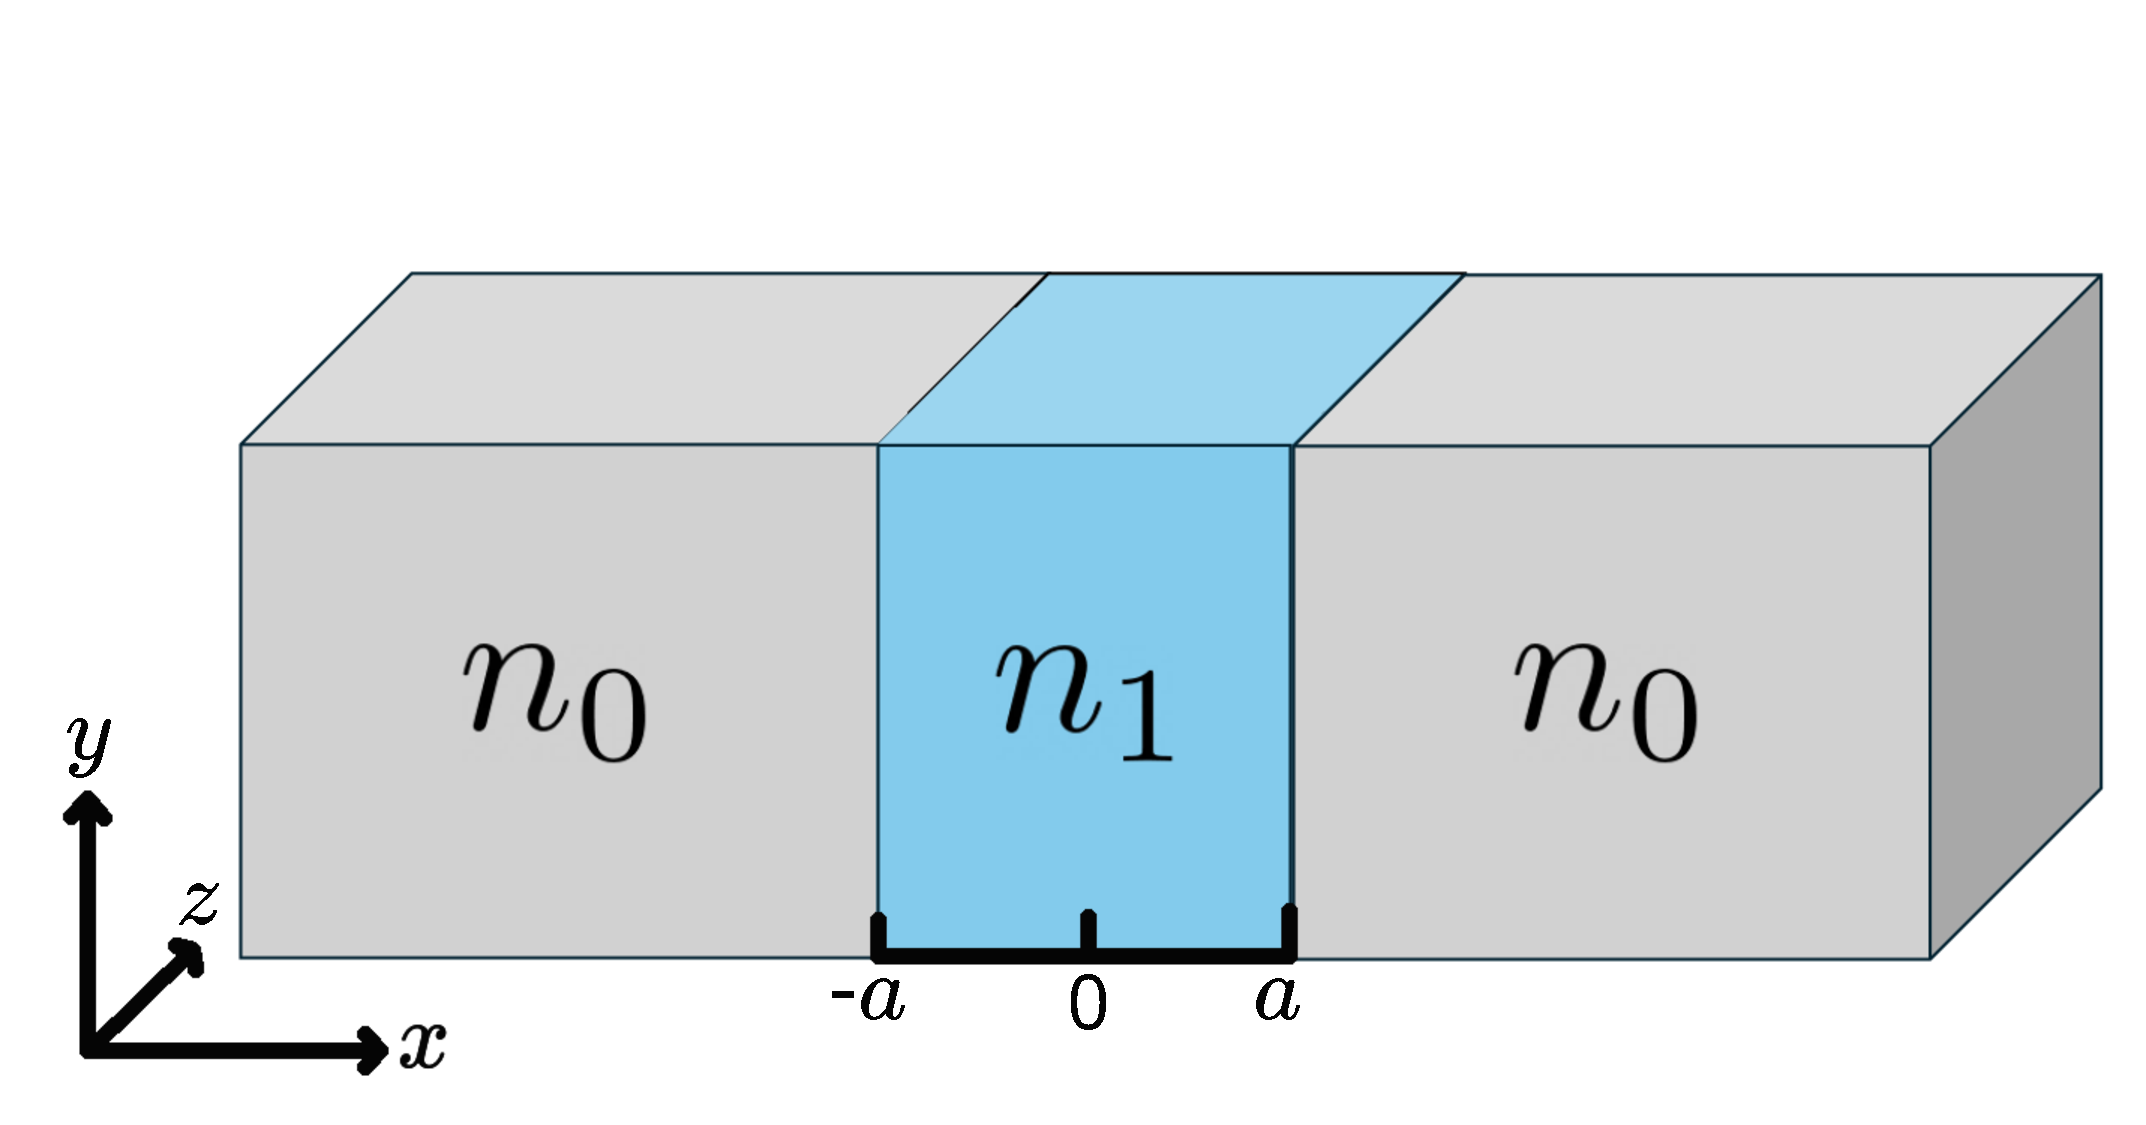
\includegraphics[width=0.6\linewidth]{media/slab.pdf}
	\caption[Forma de una guía de onda tipo losa.]{Forma de una guía de onda tipo losa. En las direcciones $\mathbf{\hat{y}}$ (vertical) y $\mathbf{\hat{z}}$ (hacia dentro de la página) la estructura es invariante.}
\end{figure}

Dado que $\nabla n^2 = \textbf{0}$ para $|x| \neq a$, los lados derechos de las ecuaciones (\ref{eqn:helmholz}) y (\ref{eqn:helmholzH}) son de tipo Helmholz. Definiendo $\Psi = \{E_z, H_z\} $:
\begin{align*}
	(\nabla_\perp^2  + k_0^2n^2 - k_z^2) \Psi  &=  \frac{d^2\Psi}{dx^2} + (k_0^2n^2 - k_z^2) \Psi  = 0.
\end{align*}

Como $n(x)=n(-x)$, las soluciones $\Psi$ deben ser pares o impares. En efecto, si $\Psi(x)$ es solución, el cambio $x\to x'=-x$ implica que $\Psi(-x)=\pm \Psi(x)$, pues $\Psi(x)$ es un campo real.

Para encontrar soluciones cuya energía esté localizada en la guía de onda y que decaiga fuera de ella, se impondrá $k_0^2n_0^2 \le k_z^2 \le k_0^2n_1^2$. Se hace natural definir $\alpha^2\equiv k_0^2n_1^2-k_z^2$ y $\beta^2\equiv k_z^2 - k_0^2n_0^2$. Con todo esto, 
\begin{equation*}
	\Psi_s = \left\{\begin{matrix}
	\Psi_{s1}\cos(\alpha x), & |x|\le a
	\\
	\Psi_{s0}e^{-\beta|x|}, & |x|>a
	\end{matrix}\right.
\end{equation*}

\begin{equation*}
	\nabla_\perp \Psi_s = \left\{\begin{matrix}
	-\hat{\textbf{x}}\alpha\Psi_{s1}\sin(\alpha x), & |x|\le a
	\\
	-\hat{\textbf{x}}\frac{|x|}{x}\beta\Psi_{s0}e^{-\beta|x|}, & |x|>a
	\end{matrix}\right.
\end{equation*}
Por lo que las componentes verticales $E_y$ y $H_y$ pares se escriben debido a la ecuación (\ref{eqn:transversal}) como:
\begin{equation*}
	\begin{aligned}[c]
	 E_y &= \frac{i \omega\mu_0}{k_0^2n^2-k_z^2} \left\{\begin{matrix}
	 \alpha H_{s1}\sin(\alpha x),	 & |x|\le a
	 \\
	 \frac{|x|}{x}\beta H_{s0}e^{-\beta|x|}, & |x|>a
	 \end{matrix}\right.
\end{aligned} 
\quad
	\begin{aligned}[c]
	 H_y &= \frac{-i\omega \epsilon_0 n^2}{k_0^2n^2-k_z^2} \left\{\begin{matrix}
	 \alpha E_{s1}\sin(\alpha x),	& |x|\le a
	 \\
	 \frac{|x|}{x}\beta E_{s0}e^{-\beta|x|}, & |x|>a
	 \end{matrix}\right.
\end{aligned} 
\end{equation*}
Por otro lado, las soluciones impares tienen la forma
\begin{equation*}
	\Psi_a = \left\{\begin{matrix}
	\Psi_{a1}\sin(\alpha x), & |x|\le a
	\\
	\Psi_{a0}e^{-\beta|x|}, & |x|>a
	\end{matrix}\right.
\end{equation*}
\begin{equation*}
	\nabla_\perp \Psi_a = \left\{\begin{matrix}
	\hat{\textbf{x}}\alpha\Psi_{a1}\cos(\alpha x), & |x|\le a
	\\
	-\hat{\textbf{x}}\frac{|x|}{x}\beta\Psi_{a0}e^{-\beta|x|}, & |x|>a
	\end{matrix}\right.
\end{equation*}
Por lo que $E_y$ y $H_y$ se escriben como:
\begin{equation*}
	\begin{aligned}[c]
	 E_y &= \frac{i\omega\mu_0}{k_0^2n^2-k_z^2} \left\{\begin{matrix}
	 -\alpha H_{a1}\cos(\alpha x)	, & |x|\le a
	 \\
	 \frac{|x|}{x}\beta H_{a0}e^{-\beta|x|}, & |x|>a
	 \end{matrix}\right.
\end{aligned} 
\quad
	\begin{aligned}[c]
	 H_y &= \frac{i\omega \epsilon_0 n^2}{k_0^2n^2-k_z^2} \left\{\begin{matrix}
	  \alpha E_{a1}\cos(\alpha x),	 & |x|\le a
	 \\
	 -\frac{|x|}{x}\beta E_{a0}e^{-\beta|x|}, & |x|>a
	 \end{matrix}\right.
\end{aligned} .
\end{equation*}
Imponiendo continuidad de las componentes tangenciales $E_y$, $E_z$, $H_y$ y $H_z$:
\begin{equation*}
	\begin{aligned}[c]
	 E_{s1}\cos(\alpha a) = E_{s0}e^{-\beta a},
	 \\	 
	 H_{s1}\cos(\alpha a) = H_{s0}e^{-\beta a},
	 \\
	 	  n_1 ^2 E_{s1}\sin(\alpha a)/\alpha = -n_0^2 E_{s0}e^{-\beta a}/\beta,
	  \\
	  H_{s1}\sin(\alpha a)/\alpha = - H_{s0}e^{-\beta a}/\beta,
\end{aligned} 
\quad
	\begin{aligned}[c]
		 E_{a1}\sin(\alpha a) = E_{a0}e^{-\beta a},
	 	   \\
	 H_{a1}\sin(\alpha a) = H_{a0}e^{-\beta a},
	 \\
	  n_1 ^2 E_{a1}\cos(\alpha a)/\alpha = n_0^2 E_{a0}e^{-\beta a}/\beta,
	 	 \\
	  H_{a1}\cos(\alpha a)/\alpha = H_{a0}e^{-\beta a}/\beta.
\end{aligned} 
\end{equation*}
Buscando soluciones no triviales se tiene que:
\begin{equation*}
	\left[\frac{\cos(\alpha a)}{\beta a} + \frac{\sin(\alpha a)}{\alpha a}\right] \left[n_0^2 \frac{\cos(\alpha a)}{\beta a} + n_1^2\frac{\sin(\alpha a)}{\alpha a} \right]
	 \left[ \frac{\sin(\alpha a)}{\beta a} - \frac{\cos(\alpha a)}{\alpha a}\right]\left[ n_0^2\frac{\sin(\alpha a)}{\beta a} - n_1^2\frac{\cos(\alpha a)}{\alpha a}\right] = 0
\end{equation*}
Se distinguirá dos tipos de condiciones:
\begin{itemize}
	\item Modos TE:\begin{align}
	\frac{\cos(\alpha a)}{\beta a} + \frac{\sin(\alpha a)}{\alpha a}&= 0, \label{eqn:TEsim}
	\\
	 \frac{\sin(\alpha a)}{\beta a} - \frac{\cos(\alpha a)}{\alpha a} &= 0. \label{eqn:TEanti}
	\end{align}
	\item Modos TM:\begin{align}
	n_0^2 \frac{\cos(\alpha a)}{\beta a} + n_1^2\frac{\sin(\alpha a)}{\alpha a}  &= 0, \label{eqn:TMsim}
	\\
	 n_0^2\frac{\sin(\alpha a)}{\beta a} - n_1^2\frac{\cos(\alpha a)}{\alpha a} &= 0. \label{eqn:TManti}
	\end{align}
\end{itemize}
Asumiendo $\alpha$, $\beta$ y $k_z$ conocidos, las amplitudes deben cumplir las relaciones:
\begin{equation*}
	\begin{aligned}[c]
	E_{s1} \left[n_0^2 \frac{\cos(\alpha a)}{\beta a}+n_1 ^2 \frac{\sin(\alpha a)}{\alpha a}\right] = 0,
		\\
	H_{s1} \left[\frac{\cos(\alpha a)}{\beta a} + \frac{\sin(\alpha a)}{\alpha a} \right] = 0,
\end{aligned} 
\quad\quad
	\begin{aligned}[c]
	E_{a1} \left[ n_0^2\frac{\sin(\alpha a)}{\beta a} - n_1^2\frac{\cos(\alpha a)}{\alpha a}\right] = 0,
		\\
	H_{a1} \left[ \frac{\sin(\alpha a)}{\beta a} - \frac{\cos(\alpha a)}{\alpha a}\right] = 0.
\end{aligned} 
\end{equation*}
Las ecuaciones superiores imponen que $E_1 = 0$ cuando se satisface la condición de modos TE. Análogamente, las ecuaciones inferiores imponen $H_1 = 0$ en el caso de modos TM. Efectivamente, los nombres TE y TM se han puesto por transversal eléctrico y transversal magnético, respectivamente.
Un corolario para los modos TE es que $E_z = E_x = 0$ por lo que la polarización del campo eléctrico será exclusivamente en la dirección $\hat{\textbf{y}}$. Así mismo, sólo un haz polarizado en $\hat{\textbf{x}}$ podría excitar un modo TM, por lo que en un experimento se debe tener esto presente: un condición inicial arbitraria se propagará como una combinación lineal de los modos TE y TM que soporte la guía.

\subsection{Soluciones gráficas y comparación entre modos TE y TM}

Usando las dos ecuaciones de modos TE junto a la restricción $(\alpha a)^2 + (\beta a)^2 = k_0^2 a^2(n_1^2 - n_0^2) \equiv V^2$ es posible obtener soluciones gráficas para las constantes de propagación $k_z$ a partir de las intersecciones $(\alpha a, \beta a)$. 

\begin{figure}[H]
	\centering
	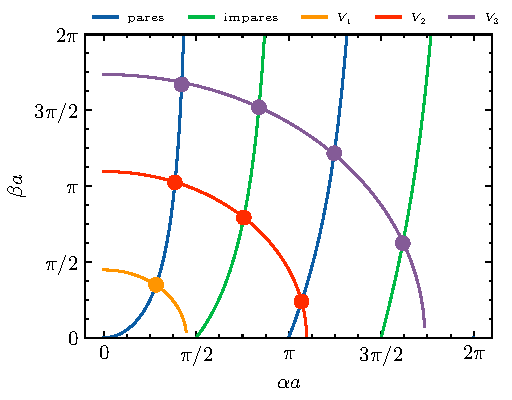
\includegraphics[width=0.7\linewidth]{media/slabgraphical.pdf}
	\caption[Soluciones gráficas de los modos TE]{Soluciones gráficas de los modos TE. A mayor contraste $\Delta n = n_1-n_0$, mayor cantidad de modos guiados soporta la guía de onda.}
\end{figure}

\begin{figure}[H]
	\centering
	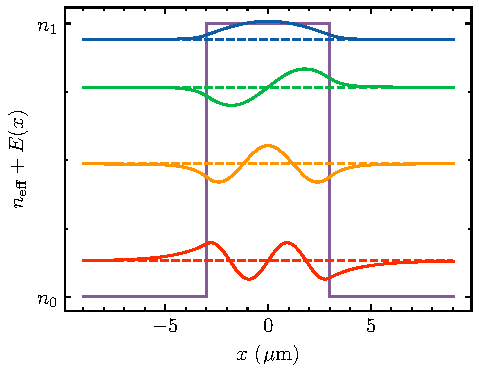
\includegraphics[width=0.7\linewidth]{media/TETMfields.pdf}
	\caption[Soluciones gráficas de los modos TE]{Soluciones gráficas de los modos TE. A mayor contraste $\Delta n = n_1-n_0$, mayor cantidad de modos guiados soporta la guía de onda.}
\end{figure}

La condición de corte (\textit{cutoff}) en guías de onda es equivalente a que la energía deje de decaer en la región $|x| > a$, es decir, se debe cumplir que $\beta a \to 0$. 
Los modos simétricos o pares cumplen esta condición para $\sin(V) = 0$, lo que implica que $V = m \pi$, con $m$ entero. En particular, considerando $m=0$  y barriendo $n_1 \to n_0$, siempre existen al menos dos modos, uno TE y otro TM hasta que $n_1 < n_0$.  
Los modos antisimétricos o impares deben cumplir por su parte que $\cos(V) = 0$, lo que implica que $V = (m\pi \pm \pi/2)$. De esta condición se deduce que el primer par de modos exictados ($m=0$) existe siempre que $\lambda \le \lambda_c \equiv 4a\sqrt{n_1^2-n_0^2}$. Escrito de forma compacta para el $m$-ésimo modo:
\begin{align*}
	 (\lambda_c)_m = \frac{4a}{m-1}  \sqrt{n_1^2-n_0^2}
\end{align*}

\section{Soluciones analíticas para fibra óptica circular}
En la sección anterior se estudió el sistema más sencillo en el que se puede hablar de guías de onda dieléctricas. El siguiente paso en complejidad consiste en guías de onda circulares. Para ello, se considerará que el índice de refracción varía radialmente según 
\begin{equation}
	n( \rho ) = 
	\left\{\begin{matrix}
	n_1, \quad \text{si } \rho \le a
	\\
	n_0, \quad \text{si } \rho > a
	\end{matrix}\right.
	,\nonumber
\end{equation}
donde la tupla $(\rho, \phi, z)$ define las coordenadas cilíndricas a usar, más apropiadas para este problema. 
Al considerar las componentes longitudinales $\Psi$ = $\{E_z, H_z\}$ del campo eléctrico y magnético y  si se utiliza el método de separación de variables con $\Psi =  R(\rho)\Phi(\phi) e^{ik_z z} $,  las ecuaciones (\ref{eqn:helmholz}) y (\ref{eqn:helmholzH}) toman la forma:

\begin{align}
	\left[\frac{\partial^2}{\partial \rho^2} + \frac{\partial}{\rho\partial \rho} + \frac{\partial^2}{\rho^2\partial \phi^2} +\left( k_0^2n^2 - k_z^2 \right)\right]  R(\rho)\Phi(\phi) = 0
	\nonumber
	\\
\rho^2\frac{d^2 R}{Rd\rho^2} + \rho\frac{dR}{Rd\rho} + \rho^2\left( k_0^2n^2 - k_z^2 \right) + \underbrace{\frac{d^2 \Phi}{\Phi d\phi^2}}_{-\ell^2} = 0
\nonumber
\\
\therefore \Phi(\phi) = A e^{i\ell\phi}
\nonumber
\end{align}
Imponiendo condiciones de periodicidad $\Phi(\phi)=\Phi(\phi + 2\pi)$, se tiene necesariamente que $\ell$ es un número entero. Por consiguiente, la ecuación para $R(\rho)$ es de tipo Bessel entera, por lo que buscando soluciones tales que $k_0^2 n_0^2 < \beta_z^2 < k_0^2 n_1^2$ y definiendo nuevamente $\alpha^2 \equiv k_0^2n_1^2 - k_z^2$ y $\beta^2\equiv k_z^2 - k_0^2n_0^2$ se tiene:
\begin{align}
	\frac{d^2 R}{d\rho^2} + \frac{1}{\rho}\frac{dR}{d\rho} + \left( k_0^2n^2 - k_z^2 -\frac{\ell^2}{\rho^2}\right)R  = 0
	\nonumber
	\\
	\therefore R(\rho) = 
	\left\{
	\begin{matrix}	
	C_1 J_\ell (\alpha\rho) + D_1 Y_\ell (\alpha\rho), \quad \text{si } \rho \le a  
	\\
	C_2 K_\ell (\beta\rho) + D_2 I_\ell (\beta\rho), \quad \text{si } \rho > a  
	\end{matrix}
	\right.
	. \nonumber
\end{align}
Necesariamente se debe imponer $D_1 = D_2 = 0$ para que la solución sea finita para $\rho = 0$ y para $\rho \to +\infty$. Es decir, la parte radial de la solución es
\begin{align*}
 R(\rho) = 
	\left\{
	\begin{matrix}	
	C_1 J_\ell (\alpha\rho), \quad \text{si } \rho \le a  
	\\
	C_2 K_\ell (\beta\rho), \quad \text{si } \rho > a  
	\end{matrix}
	\right.
	. \nonumber
\end{align*}
En este caso, para imponer las condiciones de continuidad en $\textbf{E}_{||} = E_\phi \boldsymbol{\hat{\phi}} + E_z \hat{\textbf{z}}$ y $\textbf{H}_{||}= H_\phi \hat{\boldsymbol{\phi}} + H_z \hat{\textbf{z}}$, se hace necesario relacionar el resto de componentes del campo con $E_z$ y $H_z$ para lo cual se usará la ecuación (\ref{eqn:transversal}). 

Como 
\begin{equation*}
	\nabla_\perp \Psi =
	\left\{	
	\begin{matrix}
		\Psi_0^1\left[\boldsymbol{\hat{\rho}}\alpha J'_\ell (\alpha \rho) + i \boldsymbol{\hat{\phi}} \ell J_\ell (\alpha \rho)/\rho\right] e^{i\ell\phi} e^{i k_z z}, \quad \text{si } \rho \le a  
		\\
		\Psi_0^0\left[\boldsymbol{\hat{\rho}}\beta K'_\ell (\beta\rho) +i \boldsymbol{\hat{\phi}}\ell K_\ell (\alpha \rho)/\rho \right]e^{i\ell\phi} e^{i k_z z} , \quad \text{si } \rho > a  
	\end{matrix}
	\right.
\end{equation*}

Separando por componentes y reemplazando:
\begin{align*}
		H_z &=  e^{i\ell\phi}e^{i k_z z}
	  	 \left\{
		\begin{matrix}	  	 
	  	 H_0^1 J_\ell (\alpha \rho), \quad \text{si } \rho \le a  
	  	 \\
	  	 H_0^0 K_\ell (\beta \rho), \quad \text{si } \rho > a  
	  	 \end{matrix}
	  	 \right.	
		\\
	  	 H_r &= \frac{i e^{i\ell\phi}e^{i k_z z} }{k_0^2 n^2 - k_z^2}
	  	 \left\{
		\begin{matrix}	  	 
	  	  k_z \alpha H_0^1 J'_\ell (\alpha \rho) - i\omega \epsilon_0 n^2\ell E_0^1 J_\ell (\alpha \rho)/\rho, \quad \text{si } \rho \le a  
	  	 \\
	  	 k_z \beta H_0^0  K'_\ell (\beta \rho) - i\omega \epsilon_0 n^2\ell E_0^0 K_\ell (\beta \rho)/\rho  , \quad \text{si } \rho > a  
	  	 \end{matrix}
	  	 \right.
	  	 \\
		H_\phi &= \frac{ie^{i\ell\phi} e^{i k_z z}}{k_0^2 n^2 - k_z^2}
		\left\{
		\begin{matrix}
			ik_z\ell H_0^1  J_\ell (\alpha \rho)/\rho + \omega \epsilon_0 n^2  \alpha E_0^1 J'_\ell (\alpha \rho), \quad \text{si } \rho \le a  
			\\
			ik_z \ell H_0^0  K_\ell (\beta \rho)/\rho + \omega \epsilon_0 n^2 \beta E_0^0  K'_\ell (\beta \rho), \quad \text{si } \rho > a  
		\end{matrix}
		\right.
		\\
		E_z &= e^{i\ell\phi} e^{i k_z z}
	  	 \left\{
		\begin{matrix}	  	 
	  	 E_0^1 J_\ell (\alpha \rho), \quad \text{si } \rho \le a  
	  	 \\
	  	 E_0^0 K_\ell (\beta \rho), \quad \text{si } \rho > a  
	  	 \end{matrix}
	  	 \right.	
		\\
	E_r &= \frac{i e^{i\ell\phi} e^{i k_z z} }{k_0^2 n^2 - k_z^2}
	  	 \left\{
		\begin{matrix}	  	 
	  	  k_z \alpha E_0^1 J'_\ell (\alpha \rho)+i\omega \mu_0 \ell H_0^1 J_\ell (\alpha \rho)/\rho , \quad \text{si } \rho \le a  
	  	 \\
	  	 k_z \beta E_0^0  K'_\ell (\beta \rho) +i\omega \mu_0 \ell H_0^0 K_\ell (\beta \rho)/\rho, \quad \text{si } \rho > a  
	  	 \end{matrix}
	  	 \right.
	\\
	E_\phi &= \frac{i e^{i\ell\phi} e^{i k_z z}}{k_0^2 n^2 - k_z^2}
		\left\{
		\begin{matrix}
			ik_z \ell E_0^1   J_\ell (\alpha \rho)/\rho -\omega \mu_0  \alpha H_0^1  J'_\ell (\alpha \rho), \quad \text{si } \rho \le a  
			\\
			ik_z \ell E_0^0   K_\ell (\beta \rho)/\rho -\omega \mu_0 \beta H_0^0   K'_\ell (\beta \rho) , \quad \text{si } \rho > a  
		\end{matrix}
		\right.
\end{align*}

Ahora sí, imponiendo continuidad en $z$ y $\phi$:
\begin{align}
	H_0^{1} J_\ell(\alpha a) &= H_0^{0} K_\ell (\beta a)
	\label{eqn:cont1}
	\\
	E_0^{1} J_\ell(\alpha a) &= E_0^{0} K_\ell (\beta a)
	\label{eqn:cont2}
	 \\
	 -\omega \epsilon_0 n_1^2  \alpha\beta^2 a E_0^1 J'_\ell (\alpha a)-ik_z\ell \beta^2 H_0^1  J_\ell (\alpha a)
	 &= \omega \epsilon_0 n_0^2 \alpha^2 \beta a E_0^0 K'_\ell (\beta a)+ik_z\ell \alpha^2H_0^0  K_\ell (\beta a)
	 \label{eqn:cont3}
	 \\
	 -ik_z \ell \beta^2 E_0^1   J_\ell (\alpha a) + \omega \mu_0  \alpha \beta^2 a H_0^1  J'_\ell (\alpha a) &=
	 ik_z \ell \alpha^2 E_0^0   K_\ell (\beta a) -\omega \mu_0  \alpha^2 \beta a H_0^0  K'_\ell (\beta a)
	 \label{eqn:cont4}
\end{align}
Buscando soluciones no triviales:
\begin{align*}
	\left|\begin{matrix}
		K_\ell(\beta a) & -J_\ell(\alpha a) & 0 & 0
		\\
		0 & 0 & K_\ell(\beta a) & -J_\ell(\alpha a)
		\\
		ik_z\ell \alpha^2 K_\ell (\beta a) & ik_z\ell\beta^2 J_\ell (\alpha a) & \omega \epsilon_0 n_0^2  \alpha^2 \beta a K'_\ell (\beta a) & \omega \epsilon_0 n_1^2  \alpha \beta^2 a J'_\ell (\alpha a)
		\\
		\omega \mu_0  \alpha^2 \beta a   K'_\ell (\beta a) &  \omega \mu_0  \alpha \beta^2 a J'_\ell (\alpha a) & -ik_z \ell \alpha^2 K_\ell (\beta a) &  -ik_z \ell \beta^2  J_\ell (\alpha a)
	\end{matrix}\right|
	=
0
\end{align*}
Finalmente, la ecuación trascendental que satifacen $\alpha$, $\beta$ y $k_z$ es:
\begin{equation}
	\left( \frac{J_\ell'(\alpha a)}{\alpha a J_\ell(\alpha a)} + \frac{K_\ell'(\beta a)}{\beta a K_\ell(\beta a)} \right)\left( n_1^2\frac{J_\ell'(\alpha a)}{\alpha a J_\ell(\alpha a)} + n_0^2\frac{K_\ell'(\beta a)}{\beta a K_\ell(\beta a)} \right) = \ell^2 \left[ \left(\frac{1}{\alpha a}\right)^2 + \left(\frac{1}{\beta a}\right)^2 \right]^2 \left( \frac{k_z}{k_0} \right)^2 . \label{eqn:fiber_trascendental}
\end{equation}

Dado que, en principio, los valores de $k_z$ ya están determinados por la ecuación anterior, es posible obtener dos relaciones entre $H_0^1$ y $E_0^1$:
\begin{align}
\frac{E_0^1}{H_0^1} &=  -\frac{i k_z \ell}{\omega\epsilon_0}\left[ \left(\frac{1}{\alpha a}\right)^2 + \left(\frac{1}{\beta a}\right)^2 \right]  \left[ n_1^2 \frac{J'_\ell(\alpha a)}{\alpha a J_\ell(\alpha a)} + n_0^2 \frac{K'_\ell(\beta a)}{\beta a K_\ell(\beta a)} \right]^{-1} \label{eqn:fiber_polarization_E},
\\
\frac{H_0^1}{E_0^1} &=  \frac{i k_z \ell}{ \omega\mu_0}\left[ \left(\frac{1}{\alpha a}\right)^2 + \left(\frac{1}{\beta a}\right)^2 \right]  \left[ \frac{J'_\ell(\alpha a)}{\alpha a J_\ell(\alpha a)} + \frac{K'_\ell(\beta a)}{\beta a K_\ell(\beta a)} \right]^{-1} \label{eqn:fiber_polarization_H}.
\end{align}
Tomando raíz cuadrada al cociente de las ecuaciones (\ref{eqn:fiber_polarization_E}) y (\ref{eqn:fiber_polarization_H}) se tiene:

\begin{equation}
	\frac{E_0^1}{H_0^1} = i \sqrt{\frac{\mu_0}{\epsilon_0}} \frac{\sqrt{ \frac{J'_\ell(\alpha a)}{\alpha a J_\ell(\alpha a)} + \frac{K'_\ell(\beta a)}{\beta a K_\ell(\beta a)}}}{\sqrt{n_1^2 \frac{J'_\ell(\alpha a)}{\alpha a J_\ell(\alpha a)} + n_0^2 \frac{K'_\ell(\beta a)}{\beta a K_\ell(\beta a)}}}.
	\label{eqn:fiber_polarization_simplified}
\end{equation}

\subsection{Modos TE y TM}
El caso más sencillo de estudiar es imponiendo $\ell = 0$. La ecuación (\ref{eqn:fiber_trascendental}) implica:
\begin{align*}
	\frac{J'_{0}(\alpha a)}{\alpha a J_0(\alpha a)} + \frac{K'_0(\beta a)}{\beta a K_0(\beta a)}&=  0, \quad \text{(modos TE)}
	\\
	n_1^2\frac{J'_{0}(\alpha a)}{\alpha a J_0(\alpha a)} + n_0^2 \frac{K'_0(\beta a)}{\beta a K_0(\beta a)} &= 0, \quad \text{(modos TM)}
\end{align*}

De la ecuación (\ref{eqn:fiber_polarization_simplified}) es directo notar que la condiciones de modos transversales que las componentes longitudinales se hacen cero en los casos respectivos: $H_0^1 = 0$ para TE y $E_0^1 = 0$ para TM.

Las condiciones de corte se dan cuando $\beta a \to 0$. Utilizando las expresiones asintóticas para las funciones de Bessel con argumentos pequeños y sus relaciones de recurrencia, se tiene
\begin{align*}
	\frac{\alpha a J_0(\alpha a)}{J_1(\alpha a)}  = -\frac{\beta a K_{0}(\beta a)} {K_1(\beta a)} \approx (\beta a)^2\ln\left(\frac{\beta a e^\gamma}{2}\right) \to 0,
\end{align*}
por lo que se hace necesario que $\left. J_0(\alpha a)\right|_{\alpha a \to V} = 0$. Denotando $x_{0,m}=$ 2.405,  5.520,  8.654, $\cdots$ al $m$-ésimo cero de la funcion $J_0(x)$, la longitud de onda de corte está dada por 
\begin{equation}
(\lambda_c)_{0,m} = 2\pi a \frac{\sqrt{n_1^2 - n_0^2}}{x_{0,m}}, \quad\text{(modos TE y TM).}
\end{equation} Contrario al caso de la guía de onda tipo losa, en fibras ópticas se hace necesario estar bajo un umbral de corte máximo $(\lambda_c)_{0,1}$ no nulo para que los modos TE o TM existan.

%\begin{figure}[H]
%	\centering
%	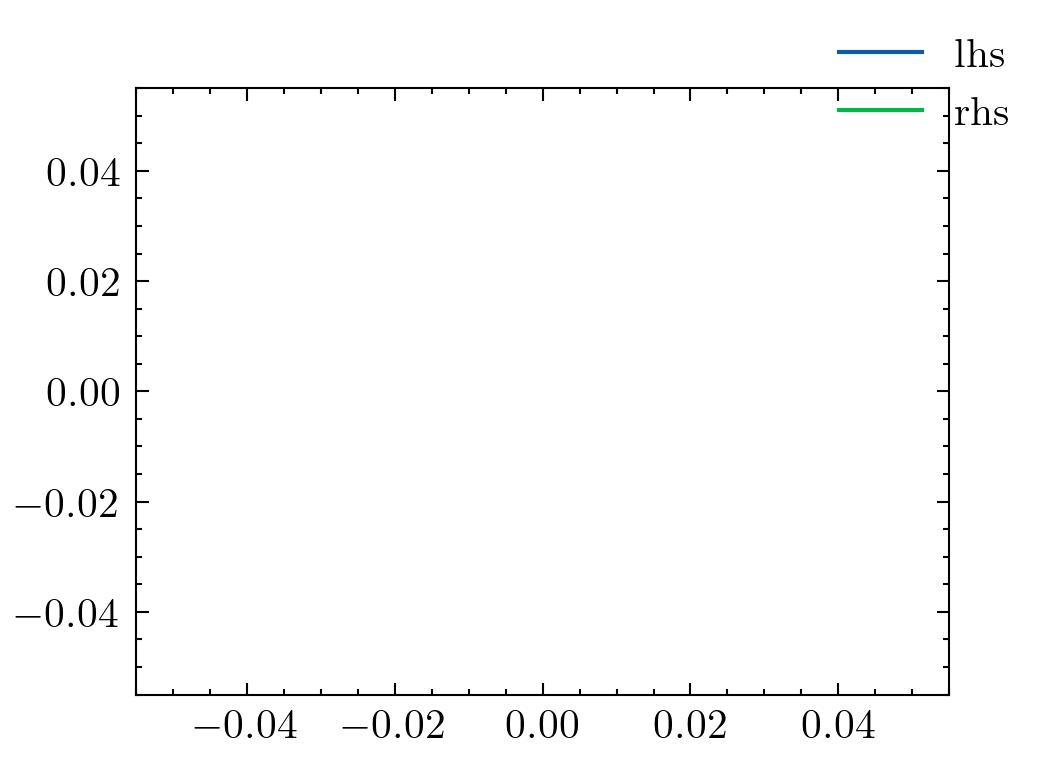
\includegraphics[width=0.7\linewidth]{media/fibergraphical}
%\end{figure}

\subsection{Modos HE y EH}
Interpretando la ecuación (\ref{eqn:fiber_trascendental}) como una cuadrática en $J_\ell'(\alpha a)/\alpha a J_\ell(\alpha a)$:
\begin{align*}
	\frac{J_\ell'(\alpha a)}{\alpha a J_\ell(\alpha a)} &= -\left(\frac{n_1^2+n_0^2}{2n_1^2}\right) \frac{K_\ell'(\beta a)}{\beta a K_\ell(\beta a)}\pm\sqrt{\left(\frac{n_1^2-n_0^2}{2n_1^2}\right)^2\left(\frac{K_\ell'(\beta a)}{\beta a K_\ell(\beta a)}\right)^2+ \left( \frac{ k_z \ell}{ k_0 n_1} \right)^2\left[ \left(\frac{1}{\alpha a}\right)^2 + \left(\frac{1}{\beta a}\right)^2 \right]^2 }
\end{align*}

Haciendo uso de las relaciones de recurrencia de las funciones de Bessel $J_\ell(r)$,  es posible obtener dos tipos de soluciones que suelen ser llamadas HE y EH debido al campo longitudinal con maor peso:
\begin{align}
		\frac{J_{\ell-1}(\alpha a)}{\alpha a J_\ell(\alpha a)} &= -\left(\frac{n_1^2+n_0^2}{2n_1^2}\right) \frac{K_\ell'(\beta a)}{\beta a K_\ell(\beta a)}+\frac{\ell}{(\alpha a)^2}-\sqrt{\Delta}, \quad \text{(modos HE)}
		\label{eqn:HE}
	\\
		\frac{J_{\ell+1}(\alpha a)}{\alpha a J_\ell(\alpha a)} &= \left(\frac{n_1^2+n_0^2}{2n_1^2}\right) \frac{K_\ell'(\beta a)}{\beta a K_\ell(\beta a)}+\frac{\ell}{(\alpha a)^2}-\sqrt{\Delta}, \quad \text{(modos EH)}
		\label{eqn:EH}
		\\
		\Delta &= \left(\frac{n_1^2-n_0^2}{2n_1^2}\right)^2\left(\frac{K_\ell'(\beta a)}{\beta a K_\ell(\beta a)}\right)^2+ \left( \frac{ k_z \ell}{ k_0 n_1} \right)^2\left[ \left(\frac{1}{\alpha a}\right)^2 + \left(\frac{1}{\beta a}\right)^2 \right]^2 \nonumber
\end{align}

Para $\ell = 0$, se recuperan las relaciones obtenidas para los modos  TE$_m$ (HE$_{0m}$) y TM$_m$ (EH$_{0m}$). Para $\ell \neq 0$ se hace necesario considerar las expresiones asintóticas de las funciones de Bessel cuando $\beta a \to 0$ y $\alpha a \to V$:
\begin{align*}
	\frac{K'_\ell (x)}{xK_\ell (x)} &= -\frac{K_{\ell-1} (x)}{xK_\ell (x)}-\frac{\ell}{x^2}\approx \left\{\begin{matrix}
	\ln(xe^\gamma/2)-\frac{1}{x^2} \quad\text{si }\ell = 1
	\\
	-\frac{
	1}{2(\ell-1)}-\frac{\ell}{x^2}\quad \text{si }\ell > 1
	\end{matrix}\right. .
\end{align*}


El caso $\ell=1$ es de especial interés. La condición de modos HE se desarrolla como
\begin{align*}
	\frac{\alpha a J_1(\alpha a)}{J_0(\alpha a)} &= \left\{\left(\frac{n_1^2+n_0^2}{2n_1^2}\right) \left[ \ln\left(\frac{2}{e^\gamma \beta a}\right)+\frac{1}{(\beta a)^2} \right]+\frac{1}{(\alpha a)^2}-\sqrt{\Delta}\right\}^{-1} \to 0.
\end{align*}

Basta considerar la función $J_1(\alpha a)|_{\alpha a \to V} = 0$. Por otro lado, la condición EH elimina el cero $x=0$ del cociente $\frac{\alpha aJ_1(\alpha a)}{J_2(\alpha a)}$ lo que hace que esté ``desfasada'' respecto a la condición HE. Usando un razonamiento similar al caso $\ell =0$, las condiciones de corte son
\begin{align*}
	(\lambda_c)_{1,m} &= 2\pi a \frac{\sqrt{n_1^2 - n_0^2}}{x_{1,m}} \quad \left(\text{modos HE}_{1m}\right)
	\\
	(\lambda_c)_{1,m} &= 2\pi a \frac{\sqrt{n_1^2 - n_0^2}}{x_{1,m+1}} \quad \left(\text{modos EH}_{1m}\right)
\end{align*}
con $x_{1,m}=0$, 3.832,  7.016, 10.173, $\dots$.
En particular, el modo $\text{HE}_{11}$ siempre existe.
\begin{figure}[H]
	\centering	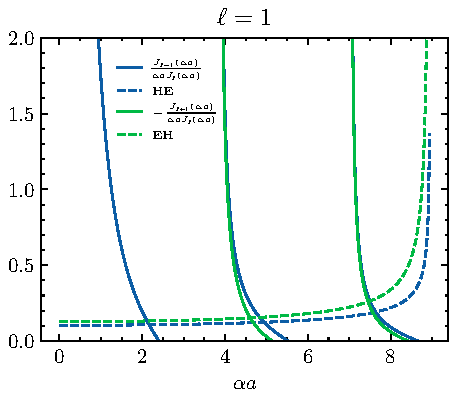
\includegraphics[width=0.6\linewidth]{media/fibergraphicalHE_EH.pdf}
\end{figure}

El caso $\ell \ge 2$ tiene un desarrollo distinto por las forma asintóticas en juego y no será relevante para esta tesis. Sin embargo, se incluyen en la Figura \ref{fig:vortices} por completitud.
\begin{figure}[H]
	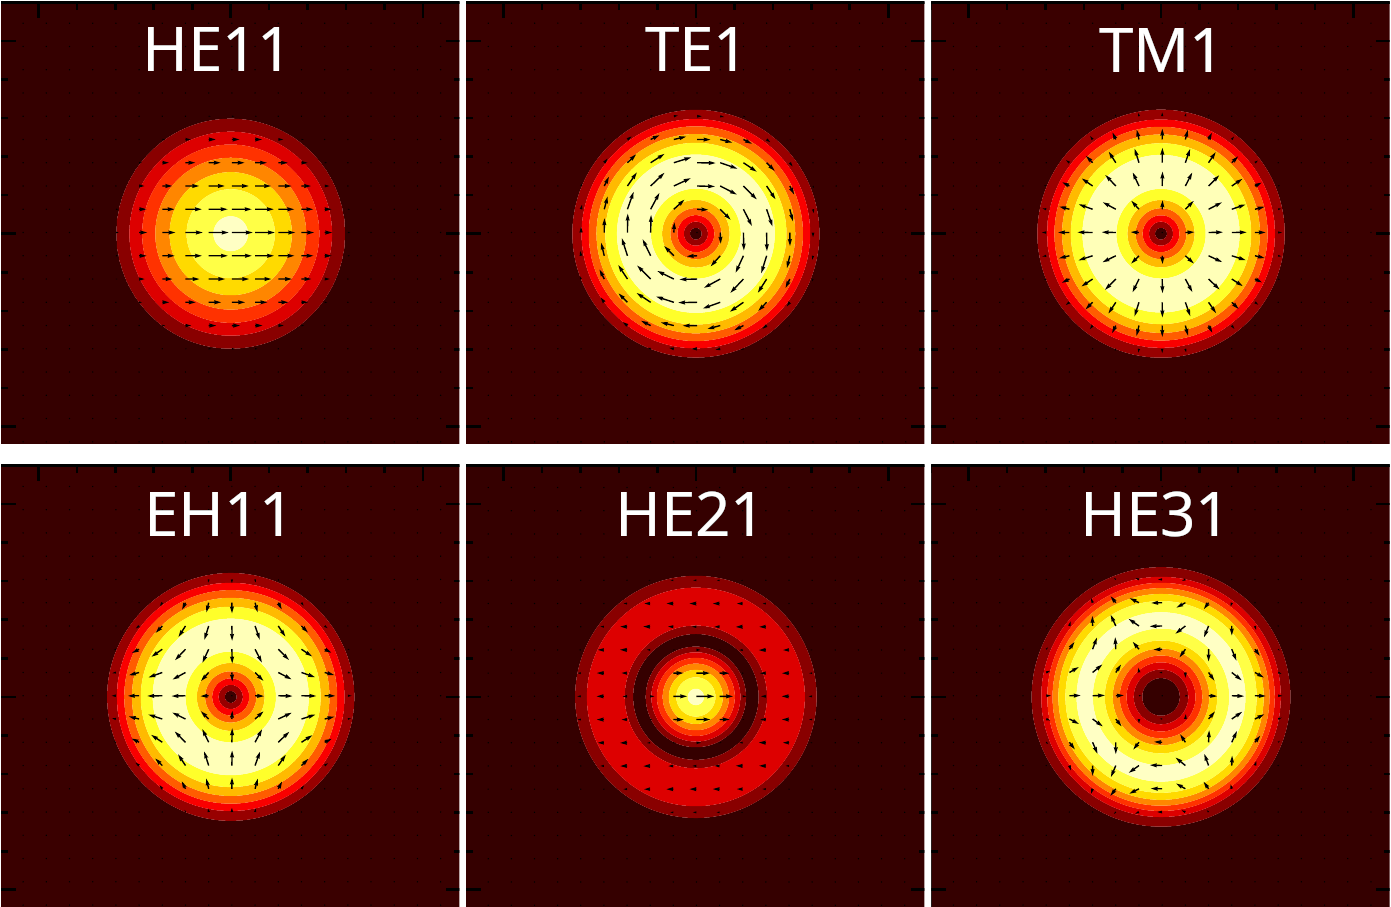
\includegraphics[width=\linewidth]{media/OAM_analitic}
		\caption{Primeros modos guiados para una guía circular o fibra óptica. \label{fig:vortices}}
\end{figure}

\section{Modos normales en guías de onda}

Si la estructura de guías de onda no varía en la dirección $z$, por separación de variables la solución para el campo eléctrico es una onda plana del tipo $\textbf{E}(\textbf{r}) = \textbf{E}_\nu(x, y) e^{i\beta_\nu z}$. A su vez, es conveniente separar el Laplaciano como $\nabla^2 \equiv \nabla_\perp^2 + \frac{\partial^2}{\partial z^2}$. De esta forma, el lado izquierdo de las ecuaciones (\ref{eqn:helmholz}), se desarrolla como:

\begin{align}
	(\nabla^2  + k_0^2n^2) \textbf{E}(\textbf{r}) &= \left(\nabla_\perp^2 + \frac{\partial^2}{\partial z^2} + k_0^2n^2\right) \textbf{E}_\nu(x, y)  e^{i\beta_\nu z} \nonumber
\\	
	&= e^{i\beta_\nu z} \nabla_\perp^2 \textbf{E}_\nu -\beta_\nu^2\textbf{E}_\nu e^{i\beta_\nu z} + k_0^2n^2 \textbf{E}_\nu  e^{i\beta_\nu z}
\nonumber	
	\\	
	&= \left[  \nabla_\perp^2  + (k_0^2n^2-\beta_\nu^2) \right]\textbf{E}_\nu  e^{i\beta_\nu z}
	\nonumber	
	\\
	&\approx
	0
	\nonumber
	\\
	\therefore
	 \left[  \nabla_\perp^2  + k_0^2n^2(x,y) \right]&\textbf{E}_\nu(x,y)  = \beta_\nu^2 \textbf{E}_\nu(x,y), \label{eqn:eigenfield}
\end{align}
donde se ha usado la aproximación de guiaje débil para anular el lado de derecho de la ecuación (\ref{eqn:helmholz}). Notemos que la ecuación (\ref{eqn:eigenfield}) es un problema de autovalores $\beta_\nu^2$ y autofunciones $\textbf{E}_\nu(x,y)$, las cuales son ortogonales (ver apéndice \ref{sec:orto}). En principio, la forma espacial del índice de refracción $n(x, y)$ puede ser arbitraria siempre y cuando que se satisfaga la condición de guiaje débil. 

\section{Teoría de modos acoplados}

\subsection{Derivación desde un principio variacional}

A partir de la ecuaciones (\ref{eqn:EfieldH}) y (\ref{eqn:HfieldE}) es posible despejar la constante de propagación $k_z$ en términos del vector de Poynting $\textbf{S} = \frac{1}{2} \text{Re}\{\textbf{E} \times \textbf{H}^*\}$, similar a lo desarrollado en la referencia \citep{haus_coupled-mode}.

\begin{equation}
	k_z = \frac{\frac{1}{4i}\iint \left(-\nabla_\perp \times \textbf{E} + i\omega \mu_0 \textbf{H} \right)\cdot\textbf{H}^* + \left(\nabla_\perp\times\textbf{H} + i\omega \varepsilon_0 n^2 \textbf{E} \right)\cdot \textbf{E}^* dxdy}{\frac{1}{4} \iint \left( \textbf{E}\times\textbf{H}^* + \textbf{E}^*\times\textbf{H}  \right) \cdot \hat{\textbf{z}} dxdy}. \label{eqn:kzprevar}
\end{equation}

De esta manera, al proponer un Ansatz en términos de superposición de modos de las guías individuales del estilo $\textbf{E} = \sum_i a_i \textbf{e}_i$, $\textbf{H} = \sum_i a_i \textbf{h}_i$, los coeficientes $a_i$ quedan indeterminados pero sujetos a minimizar la expresión para $k_z$. Notemos además que el Ansatz simplifica bastante la mencionada expresión.
\begin{align*}
	(\textbf{E}\times\textbf{H}^* + \textbf{E}^*\times\textbf{H})\cdot\hat{\textbf{z}} = \sum_{ij} a_i^*( \textbf{e}_j \times  \textbf{h}_i^* + \textbf{e}_i^* \times  \textbf{h}_j  )\cdot\hat{\textbf{z}} a_j \equiv \sum_{ij} a_i^* p_{ij} a_j
\end{align*}
\begin{align*}
	\text{integrando numerador} &= i\sum_{ij} a_i^* k_z^j (\hat{\textbf{z}}\times\textbf{e}_j )\cdot\textbf{h}_i^* a_j + a_j\left(\omega \varepsilon_0 (n^2-n_j^2) \textbf{e}_j-k_z^j \hat{\textbf{z}}\times\textbf{h}_j \right)\cdot \textbf{e}_i^* a_i^*
	\\
	&= i\sum_{ij}  a_i^*\left[ k_z^j p_{ij}  +  \omega \varepsilon_0(n^2-n_j^2) \textbf{e}_j \cdot \textbf{e}_i^* \right] a_j
\end{align*}

Definiendo 
\begin{align}
	P_{ij} &\equiv \frac{1}{4} \iint ( \textbf{e}_j \times  \textbf{h}_i^* + \textbf{e}_i^* \times  \textbf{h}_j  )\cdot\hat{\textbf{z}} dxdy,
	\\
	H_{ij} &\equiv  P_{ij} k_z^j + \frac{\omega \varepsilon_0}{4} \iint(n^2-n_j^2) \textbf{e}_j \cdot \textbf{e}_i^* dxdy.
\end{align}

Se puede escribir la expresión (\ref{eqn:kzprevar}) para la constante de propagación $k_z$ de manera compacta como un cociente de Rayleigh-Ritz:
\begin{equation}
	k_z = \frac{\sum_{ij} a_i^* H_{ij} a_j}{\sum_{ij} a_i^*P_{ij} a_j}.
\end{equation}

Diferenciando con respecto a $a_k^*$ para optimizar el valor de $k_z$ se tiene:
\begin{align}
	\frac{\partial k_z}{\partial a_k^*} &= \frac{\sum_{ij} H_{ij} a_j \delta_{ik}}{\sum_{ij} a_i^*P_{ij} a_j} - \frac{\left(\sum_{ij} a_i^* H_{ij} a_j\right) \left( 
	\sum_{ij} \delta_{ik} P_{ij} a_j \right) }{\left(\sum_{ij} a_i^*P_{ij} a_j\right)^2} = \frac{\sum_{j} \left(H_{jk}  - k_z P_{kj} \right) a_j}{\sum_{ij} a_i^* P_{ij}a_j} \overset{!}{=} 0.
\end{align}

Recuperando $k_z \to -i\frac{\partial}{\partial z}$, se obtienen las ecuaciones de $N$ modos acoplados no ortogonales:
\begin{equation}
	-i \sum_{j} P_{kj} \frac{d a_j}{dz} ´= \sum_{j} H_{kj} a_j, \text{ con }k=1,2,\dots,N \label{eqn:non-ortho-CMT-eqs}
\end{equation}
	
Claramente $P_{ij}$ es una matriz hermítica. A primera vista, puede parecer que $H_{ij}$ no es hermítica, pero veamos que sí lo es. Para ello, basta considerar la resta $H_{ij} - H_{ji}^*$ y notar que se anula:
\begin{align*}
 H_{ij} - H_{ji}^* &= P_{ij} k_z^j - P_{ji}^* k_z^i  + \frac{\omega \varepsilon_0}{4} \iint(n_i^2-n_j^2) \textbf{e}_i^* \cdot \textbf{e}_j dxdy
\\
&= \frac{1}{4} \iint (k_z^j-k_z^i)( \textbf{e}_j \times  \textbf{h}_i^* + \textbf{e}_i^* \times  \textbf{h}_j  )\cdot\hat{\textbf{z}} + \omega\varepsilon_0 (n_i^2-n_j^2) \textbf{e}_j \cdot \textbf{e}_i^* dxdy
\\
&= \frac{1}{4} \iint \left( i\nabla_\perp \times \textbf{e}_j +\omega\mu_0 \textbf{h}_j \right) \cdot \textbf{h}_i^* - \left( i\nabla_\perp \times \textbf{h}_j  - \omega\varepsilon_0n_j^2 \textbf{e}_j \right) \cdot \textbf{e}_i^*dxdy
\\
&- \frac{1}{4} \iint \left( i\nabla_\perp \times \textbf{e}_i^* +\omega\mu_0 \textbf{h}_i^*\right) \cdot \textbf{h}_j + \left(i\nabla_\perp \times \textbf{h}_i^*  + \omega\varepsilon_0n_i^2 \textbf{e}_i^* \right) \cdot \textbf{e}_jdxdy
\\
&+\frac{\omega\varepsilon_0}{4}\iint  \left(n_i^2-n_j^2\right) \textbf{e}_j \cdot \textbf{e}_i^* dxdy
\\
&= \frac{i}{4} \iint \left(\nabla_\perp\times\textbf{e}_j\right) \cdot \textbf{h}_i^*  -\left(\nabla_\perp\times\textbf{h}_j\right) \cdot \textbf{e}_i^* + \left(\nabla_\perp\times\textbf{e}_i^*\right) \cdot \textbf{h}_j - \left(\nabla_\perp\times\textbf{h}_i^*\right) \cdot \textbf{e}_j dxdy
\\
&= \frac{i}{4} \iint \nabla_\perp\cdot\left(\textbf{e}_j \times \textbf{h}_i^* +\textbf{e}_i^* \times \textbf{h}_j\right) dxdy
\\
&=
\frac{i}{4} \oint_C \left(\textbf{e}_j \times \textbf{h}_i^* +\textbf{e}_i^* \times \textbf{h}_j\right) \cdot \hat{\textbf{z}} ds
\\
&=
0,
	\end{align*}
donde se ha usado que los campos deben decaer a cero en el infinito. Las ecuaciones (\ref{eqn:non-ortho-CMT-eqs}) se pueden obtener a partir de un Principio de Mínima Acción luego de definir el Lagrangiano $L$ de tipo campo discreto de Schrödinger:
\begin{equation}
	L = -\sum_{ij}  a_i^*\left(i  P_{ij} \frac{d }{dz} + H_{ij}  \right)a_j.
\end{equation}
Los momentos generalizados de este Lagrangiano es $\Pi_k=\frac{\partial L}{\partial \dot{a_k}} = -i\sum_{j} a_j^* P_{jk}$, por lo que el Hamiltoniano $H$ asociado es
\begin{equation}
H = \sum_{j} \Pi_j \dot{a_j} - L = \sum_{ij} -ia_i^* P_{ij} \dot{a_j} + a_i^*\left(i  P_{ij} \frac{d a_j}{dz} + H_{ij} a_j \right) = \sum_{ij} a_i^* H_{ij} a_j.
\end{equation}
Variando el Lagrangiano se tiene:
\begin{align*}
	\delta L &= \sum_{ij} \frac{\partial L}{\partial a_j} \delta a_{j} +  \frac{\partial L}{\partial {a}_{i}^*} \delta {a}_{i}^* + \ \frac{\partial L}{\partial \dot{a}_{j}} \delta \dot{a}_{j} + \frac{\partial L}{\partial \dot{{a}}_{i}^*} \delta \dot{{a}}_{i}^*
	\\
	&= \sum_{ij} \left( \frac{\partial L}{\partial a_{j}} - \frac{d}{dz}\frac{\partial L}{\partial \dot{a}_{j}} \right)\delta a_{j} + \left( \frac{\partial L}{\partial {a}_{i}^*} - \frac{d}{dz}\frac{\partial L}{\partial  \dot{{a}}_{i}^*} \right)\delta {a}_{i}^* + \frac{d}{dz}\left(\frac{\partial L}{\partial \dot{a}_{j}}\delta a_{j} +  \frac{\partial L}{\partial \dot{{a}}^*_{i}}\delta {a}_{i}^*\right)
	\\	
	&\implies  \frac{d}{dz} \sum_{ij}\left(\frac{\partial L}{\partial \dot{a}_{j}}\delta a_{j} +  \frac{\partial L}{\partial \dot{{a}}_{i}^*}\delta {a}_{i}^*\right) = 0.
\end{align*}
Al considerar el par de transformaciones asociadas al grupo unitario U(1), $a_j\to a'_j = e^{i\phi}a_j$, ${a}_i^* \to {a'}_i^* = e^{-i\phi}{a}_i^*$ que dejan invariante el Lagrangiano, y si se toma una variación infinitesimal $\phi \ll 1$ se tiene $\delta a_j = i\phi a_j$ y $\delta {a}_i^* = -i\phi {a}_i^*$, por lo que la cantidad conservada, $P$, que se identifica con la potencia total del sistema es:
\begin{equation}
	P = \sum_{ij} a_i^* P_{ij} a_j = \iint \textbf{S} \cdot \hat{\textbf{z}} dxdy.  \label{eqn:power}
\end{equation}
Se tienen entonces dos cantidades conservadas en la dinámica, $H$ y $P$, que serán de utilidad para verificar la validez de soluciones numéricas a la ecuación (\ref{eqn:non-ortho-CMT-eqs}).

\subsection{Aplicaciones}
\subsubsection{Arreglo 1D de guías tipo losa}
Para los modos TE fundamentales (condición antisimétrica) y las ecuaciones (\ref{eqn:transversal}) se tiene que

\begin{align}
	\textbf{e}_{j\perp} &= \hat{\textbf{y}}\frac{i\omega\mu_0 H_{a1}}{k_0^2n_j^2 - k_z^2}\left\{ \begin{matrix}
-\alpha \cos(\alpha (x-x_j)), &|x-x_j|\le a
\\
\beta\sin(\alpha a) e^{-\beta(|x-x_j|-a)}, &|x-x_j| > a
\end{matrix}\right.
\\
\textbf{h}_{j\perp} &= \hat{\textbf{x}}\frac{ik_z^j H_{a1}}{k_0^2n_j^2 - k_z^2}\left\{ \begin{matrix}
\alpha \cos(\alpha (x-x_j)), &|x-x_j|\le a
\\
-\beta\sin(\alpha a) e^{-\beta(|x-x_j|-a)}, &|x-x_j| > a
\end{matrix}\right.
\end{align}
$x_j=jb$, con $b\ge 2a$ y $L=\int dy$. Elementos no diagonales tienen la forma:
\begin{align}
	\left(\textbf{e}_{j\perp}\times\textbf{h}_{i\perp}^*\right)\cdot \hat{\textbf{z}}
	=
	\frac{k_z^i \omega \mu_0 H_{a1}^2 \beta\sin(\alpha a)}{(k_0^2n_j^2 - k_z^2)(k_0^2n_i^2 - k_z^2)}
	\left\{
	\begin{matrix}
		 \alpha\cos(\alpha(x-x_i))e^{-\beta(|x-x_j|-a)}, & |x-x_i| \le a
		\\
		i \leftrightarrow j, & |x-x_j| \le a
		\\
		\beta \sin(\alpha a)e^{-\beta (|x-x_i|+|x-x_j|-2a)}, & \text{otro caso}
	\end{matrix}
	\right.
\end{align}

\begin{align*}
	P_{ij} &= k_z^i L \omega \mu_0 H_{a1}^2 \beta\sin^2(\alpha a)e^{-\beta b |i-j|} e^{2\beta a} \left[\frac{1}{\alpha^2(\alpha^2+\beta^2)} + \frac{e^{-2\beta a}+\beta\left(|i-j|b-2a\right)}{2\beta^4} \right]			
\end{align*}

Elementos diagonales tienen la forma:
\begin{align*}
	\left(\textbf{e}_{j\perp}\times\textbf{h}_{j\perp}^*\right)\cdot \hat{\textbf{z}}&=\frac{k_z^j\omega\mu_0 H_{a1}^2}{(k_0^2n_j^2-k_z^2)^2} \left\{ \begin{matrix}
\alpha^2\cos^2(\alpha (x-x_j)), & |x-x_j| \le a
\\
\beta^2 \sin^2(\alpha a) e^{2\beta a} e^{-2\beta|x-x_j|}, & |x-x_j|>a
\end{matrix}\right.
\end{align*}



\begin{align*}
	P_{jj} &= \frac{k_z^j \omega\mu_0H_{a1}^2 L a}{2 \alpha^2} \left[1 + \frac{\sin^2(\alpha a)}{a \beta^3 } k_0^2 \left( n_1^2 - n_0^2 \right) \right]
\end{align*}
\begin{align*}
	H_{jj} - P_{jj} k_z^j = \frac{\omega\epsilon_0}{4} \iint (n^2 - n_j^2)|\textbf{e}_j|^2 dx dy
\end{align*}

\section{Bandas y Topología en Redes Fotónicas}

Si bien es posible reformular las ecuaciones de Maxwell como un problema de autovalores en analogía a Mecánica Cuántica para plantear el Teorema de Bloch \cite{joannopoulos_photonic_2008}, en el contexto de sistemas discretos la ecuación tipo Schrödinger (\ref{eqn:CMT_mat}) con la matriz $\hat{C}$ hermítica es justificación suficiente para invocarlo: Es posible expresar las soluciones del sistema en una base de cuasimomento cuya periodicidad sea la misma que la de la matriz $\hat{C}$. En la práctica, se aplicará un Ansatz de Bloch $|a\rangle = e^{i(\lambda z + \textbf{k}\cdot \textbf{r})}|A\rangle$, con $|A\rangle$ un vector constante de la misma dimensionalidad que número de sitios en la celda unitaria de la red. De esta manera, será posible etiquetar $\lambda \equiv \lambda_n(\textbf{k})$

Para sistemas finitos, los autovalores de la matriz $\hat{C}$ tenderán a agruparse en el mismo número de bandas que cantidad de sitios por celda unitaria conformen el sistema, dado que las funciones de Wannier asociadas al Teorema de Bloch aproximan de mejor manera al sistema en cuestión a medida que aumenta el número de celdas.

\subsection{Correspondencia bulto-borde}
En sistemas hermíticos existe una correspondencia entre las propiedades de las bandas del sistema, calculadas con condiciones de borde periodicas y los autoestados de borde asociados a la matriz $\hat{C}$, calculados con condiciones de borde abiertas \cite{topobulk}.

